%%%%% SOME OPTIONS %%%%% 
\newcommand{\german}{false} % germanTrue or false --> Switch between german and english headers / titlepage
\newcommand{\coloredTitlePage}{true} % Switch between colored and BW titlepage
\newcommand{\company}{false}
\newcommand{\ECE}{true}
\newcommand{\RN}[1]{\uppercase\expandafter{\romannumeral#1}}
%%%%% Required Settings for the template %%%%%
%%%%% Configuration Package for the ThesisTemplate ECE / AEE %%%%%%
%
% Created by Mayer Florian October/2016
% v1.0

%======= DocumentClass ===========%
\documentclass[11pt, openright]{book} %Extarticle supports more FontSizes

%========= ADD Latex PACKAGES =========%
\usepackage{tabularx}         
\usepackage{parskip}%NEW
\newcolumntype{x}[1]{!{\centering\arraybackslash\vrule width #1}}
\usepackage{booktabs}
\usepackage[utf8]{inputenc} %to allow vowel mutations
\usepackage{tikz} % Schematic creator with TikZ in LaTex
\usepackage{geometry,titlesec,layout}
\usepackage{subfigure}
\usepackage{xcolor,colortbl}
%\usepackage{graphicx,rotating}
\usepackage{float}
\usepackage{epstopdf}
\usepackage[titles]{tocloft}
\usepackage{blindtext}
\usepackage{anyfontsize}
\usepackage{setspace,varwidth}
\usepackage{ifthen}
\usepackage{multicol,multirow}
\usepackage{makecell}
\usepackage{cancel}
\usepackage[stable,bottom,hang,splitrule,multiple]{footmisc}% customize footnotes
\usepackage[final]{listings}% program code listings
\usepackage[%
headtopline,plainheadtopline,% activate all lines (header and footer)
headsepline,plainheadsepline,%
footsepline,plainfootsepline,%
footbotline,plainfootbotline,%
nouppercase% auto update \..mark
]{scrlayer-scrpage}% (KOMA)

\usepackage[%
breaklinks=true,% allow line break in links
colorlinks=true,% if false: framed link
linkcolor=black,anchorcolor=black,citecolor=black,filecolor=black,%
menucolor=black,urlcolor=black]{hyperref}% hyperlinks for references

\usepackage{amssymb}
\usepackage{emptypage}
\usepackage{glossaries}
\usepackage{appendix}
\usepackage{mdframed}
\usepackage{etoolbox}
\usepackage{chngcntr} 

\usepackage{textcomp}
\usepackage{lmodern}
\usepackage[european, straightvoltages, americaninductors, oldvoltagedirection]{circuitikz}

%========= ADD TikZ PACKAGES =========%
\usetikzlibrary{matrix,calc,positioning,arrows,shapes}
\usetikzlibrary{decorations.pathreplacing}

%======= END ADD PACKAGES =======%
\geometry{a4paper,twoside,%
	%textheight=205mm, %246mm,%
	textwidth=160mm,%
	top = 3cm,
	bottom = 4.5cm,
	heightrounded=false,% round textheight to multiple of lines (avoids overfull vboxes)
	ignoreall=true,% do not include header, footer, and margins in calculations
	marginparsep=5pt,% marginpar only used for signs (centered), thus only small sep. needed
	marginparwidth=10mm,% prevent margin notes to be out of page
	hmarginratio=1:2,
	voffset = 2.25mm,
	%headheight = 16mm,
	headsep = 9mm,
	footskip = 13mm
}
\linespread{1.4}
%======= DEFINE COLORS ===========%
\definecolor{DENcol}{RGB}{35,171,196} % Department Colour


%======= Re-Define Essential Commands and store old ones ======%
\newcommand{\ChapterFont}{qag}
\newcommand{\WorkingFont}{\rmdefault}
\renewcommand{\familydefault}{\WorkingFont}
\normalfont

%======= Set Depths of TOC / TOF / TOL =======%

\renewcommand{\cftchapfont}{\bf\large\fontfamily{\sfdefault}\selectfont}
\renewcommand{\cftpartfont}{\bf\large\fontfamily{\sfdefault}\selectfont}

\ifthenelse{\equal{\german}{true}}
{
\usepackage[ngerman]{babel}
\renewcommand{\lstlistingname}{Programmcode} 
}
%====== Usefull Additional Commands =======%

% Make clickable footnote
    \newcommand{\hyperfootnote}[1][]{\def\ArgI\hyperfootnoteRelay}
    % relay to new command to make extra optional command possible
    \newcommand\hyperfootnoteRelay[2][]{\href{#1#2}{\ArgI}\footnote{\href{#1#2}{#2}}}
    % the first optional argument is now in \ArgI, the second is in #1
    %http://www.brechtdeman.com/blog/latex-clickable-footnote.html
    % Simple (no arguments)
    %    \hyperfootnote{http://www.mywebsite.com}
    % Link text (1 argument)
    %   \hyperfootnote[My website]{http://www.mywebsite.com}
    % Link text and invisible prefix (2 arguments)
    %   \hyperfootnote[My website][http://]{www.mywebsite.com}

\newcommand{\ie}{i.\,e.}
\newcommand{\Ie}{I.\,e.}
\newcommand{\eg}{e.\,g.}
\newcommand{\Eg}{E.\,g.} 

%====== Heading Commands =======%

\pagestyle{scrheadings}%
% \setlength\parindent{0cm}% no indentation for first line of new paragraph
% \raggedbottom% do not try to fill pages

% header and footer size
\setheadwidth{text}% set header width to textwidth
\setfootwidth{text}% set footer width to textwidth
\setheadtopline[textwithmarginpar]{0.25pt}% set up separator lines (greater width than text)
\setheadsepline[textwithmarginpar]{0.25pt}
\setfootsepline[textwithmarginpar]{0.25pt}
\setfootbotline[textwithmarginpar]{0.25pt}

\renewcommand*\chaptermark[1]{\markleft{\thechapter~#1}}
\renewcommand*\sectionmark[1]{\markright{\thesection~#1}} 

\clearscrheadfoot % clear everything
\ihead[]{}%
\ohead[\ShortTitle]{\footnotesize\headmark}%
%\cfoot[\footnotesize\ConfidNote]{\footnotesize\ConfidNote}%

\ofoot[\ifthenelse{\equal{\thepage}{}}{\pagemark}{--~~\pagemark~~--}]{\ifthenelse{\equal{\thepage}{}}{\pagemark}{--~~\pagemark~~--}}%

%============== Chapter / Section / Subsection Style ==== %
\titleformat{\part}[display]
   {\fontfamily{\sfdefault}\bfseries\fontsize{26}{26}\selectfont\filcenter}
   {\fontfamily{\sfdefault}\bfseries\fontsize{30}{22}\selectfont\partname{} \thepart}
   {0.5em}
   {}

\titleformat{\chapter}[display]
{\fontfamily{\sfdefault}\bfseries\fontsize{22}{22}\selectfont}%\
{
\begin{tikzpicture}[overlay]
	\node (CoolTitle) at (12,1) [opacity=0.325]{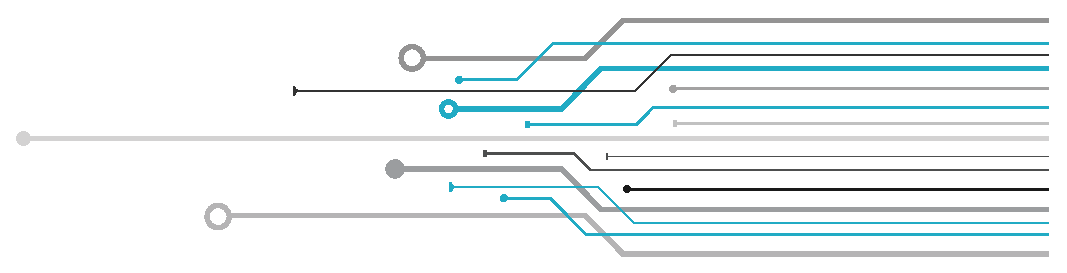
\includegraphics[scale=0.75]{LaTeX/temp_graphics/chapterBacking.eps}};
	\node (titleNumber) at ($(CoolTitle)+(3,0)$) {\textcolor{black!80}{\fontfamily{\ChapterFont}\bfseries\Large\fontsize{80}{80}\selectfont\thechapter}};
\end{tikzpicture}
}
{0.05em}%
{\vspace{0.25ex}\filleft}%

\titleformat{\section}{\Large \bfseries \sffamily}{\thesection}{1 em}{}
\titleformat{\subsection}{\large \bf \sffamily}{\thesubsection}{1 em}{}
\titleformat{\subsubsection}{\large \bf \sffamily}{\thesubsubsection}{1 em}{}

%%%% CLEAR DOUBLE-PAGE
% redefine cleardoublepage...
\makeatletter
\renewcommand{\cleardoublepage}{\clearpage\if@twoside\ifodd\c@page\else\thispagestyle{plain}\hbox{}\newpage\if@twocolumn\hbox{}\newpage\fi\fi\fi}
% ...and define empty double page (e.g., for title sheet)
\newcommand{\emptydoublepage}{\clearpage\if@twoside\ifodd\c@page\else\thispagestyle{empty}\hbox{}\newpage\if@twocolumn\hbox{}\newpage\fi\fi\fi}%
% ...and also an empty single page
\newcommand{\emptypage}{\clearpage\thispagestyle{empty}\hbox{}\newpage\if@twocolumn\hbox{}\newpage\fi}%
\makeatother

%%%%% Correct Even and Odd Pages %%%%%
\let\tmp\oddsidemargin
\let\oddsidemargin\evensidemargin
\let\evensidemargin\tmp
\reversemarginpar

% code listings
\lstloadlanguages{Bash,VHDL,Matlab,[ANSI]C,Java,[LaTeX]TeX}

\lstset{
	frame=top,frame=bottom,
	basicstyle=\fontsize{8}{8}\normalfont\sffamily,    % the size of the fonts that are used for the code
	stepnumber=1,                           % the step between two line-numbers. If it is 1 each line will be numbered
	numbersep=6pt,                         % how far the line-numbers are from the code
	tabsize=2,                              % tab size in blank spaces
	extendedchars=true,                     %
	breaklines=true,                        % sets automatic line breaking
	captionpos=t,                           % sets the caption-position to top
	mathescape=true,
	stringstyle=\color{black}\ttfamily, % Farbe der String
	showspaces=false,           % Leerzeichen anzeigen ?
	showtabs=false,             % Tabs anzeigen ?
	xleftmargin=15pt,
	framexleftmargin=14pt,
	framexrightmargin=9pt,
	framexbottommargin=5pt,
	framextopmargin=5pt,
	showstringspaces=false,      % Leerzeichen in Strings anzeigen ?
	numbers = left,
	linewidth = 150mm
}
%%%% MDBOX Setup
\mdfsetup{%
middlelinecolor=red,
middlelinewidth=2pt,
backgroundcolor=DENcol!10,
roundcorner=10pt,
topline = false,
bottomline = false,
rightline = false,
linecolor = DENcol,
linewidth = 10pt}

%%%% GET RID OF OVERFULL BOXING WARNINGS %%%%
%\overfullrule=5pt
\setlength{\headheight}{1.1\baselineskip}
\raggedbottom

%%%%%%%%%%%%%
\counterwithout{footnote}{chapter}


\usepackage{hyperref}

\makeglossaries

\makeatletter
\newcommand{\myscope}[2] % #1 = name , #2 = rotation angle
{\draw[thick,rotate=#2] (#1) circle (12pt)
 (#1) ++(-0.35,-0.1) -- ++(0.3,0.3) --++(0,-0.3)-- ++(0.3,0.3) --++(0,-0.3);
}
\newcommand{\costumPicWidth}[0]{
0.8\textwidth
}

\newcommand{\costumPlotWidth}[0]{
\textwidth
}

%\addto\extrasngerman{\def\figureautorefname{Abbildung}}
%\addto\extrasngerman{\def\equationautorefname{Gleichung}}
%\addto\extrasngerman{\def\tableautorefname{Tabelle}}

\newcommand{\V}[0]{\text{V}}
\newcommand{\mV}[0]{\text{mV}}
\newcommand{\uV}[0]{\mu\text{V}}

\newcommand{\A}[0]{\text{A}}
\newcommand{\mA}[0]{\text{mA}}
\newcommand{\uA}[0]{\mu\text{A}}

\newcommand{\s}[0]{\text{s}}
\newcommand{\ms}[0]{\text{ms}}
\newcommand{\us}[0]{\mu\text{s}}

\newcommand{\Ohms}[0]{\Omega}
\newcommand{\KOhms}[0]{\text{K}\Omega}
\newcommand{\MOhms}[0]{\text{M}\Omega}

\newcommand{\F}[0]{\text{F}}
\newcommand{\mF}[0]{\text{mF}}
\newcommand{\uF}[0]{\mu\text{F}}
\newcommand{\nF}[0]{\text{nF}}

\newcommand{\Hz}[0]{\text{Hz}}
\newcommand{\kHz}[0]{\text{kHz}}
\newcommand{\MHz}[0]{\text{MHz}}

\newcommand{\dB}[0]{\text{dB}}

\newcommand{\degree}[0]{^\circ}

\newcommand{\Mikro}[0]{\mu}
\newcommand{\Milli}[0]{\text{m}}
\newcommand{\Kilo}[0]{\text{k}}
\newcommand{\Mega}[0]{\text{M}}

\begin{document}
%%%%% ThesisTemplate ECE / AEE %%%%%%
%
% Created by Mayer Florian October/2016
% v1.0

%============== Glossary Command ==== %

\newglossaryentry{SCSS}{name=SCSS, description={Single Channel Source Separation}} 
\newglossaryentry{ITD}{name=ITD, description={Interaural Time Difference}}
\newglossaryentry{PASCSS}{name=PASCSS, description={Phase-Aware Single Channel Source Separation}}
\newglossaryentry{CASA}{name=CASA, description={Computational Auditory Scene Analysis}}
\newglossaryentry{NMF}{name=NMF, description={Non-Negative Matrix Factorization}}
\newglossaryentry{CMF}{name=CMF, description={Complex Matrix Factorization}}
\newglossaryentry{STFT}{name=STFT, description={Short-Time Fourier Transformation}}
\newglossaryentry{DTFT}{name=DTFT, description={Discrete-Time Fourier Transformation}}
\newglossaryentry{ISTFT}{name=ISTFT, description={Inverse Short-Time Fourier Transformation}}
\newglossaryentry{IBM}{name=IBM, description={Ideal Binary Mask}}
\newglossaryentry{IRM}{name=IRM, description={Ideal Ratio Mask}}
\newglossaryentry{SNR}{name=SNR, description={Signal-to-Noise Ratio}}
\newglossaryentry{DNN}{name=DNN, description={Deep neural network}}
\newglossaryentry{SVM}{name=SVM, description={Support vector machine}}
\newglossaryentry{KL-divergence}{name=KL-divergence, description={Kullback-Leibler divergence}}
\newglossaryentry{MPE}{name=MPE, description={Multipitch Estimator}} 
\newglossaryentry{PEFAC}{name=PEFAC, description={Pitch Estimation Filter with Amplitude Compression}}  
\newglossaryentry{GMM}{name=GMM, description={Gaussian mixture models}} 
\newglossaryentry{GLA}{name=GLA, description={Griffin and Lim Algorithm}}  
\newglossaryentry{MISI}{name=MISI, description={Multiple Input Spectrogram Inversion}}
\newglossaryentry{PPR}{name=PPR, description={Partial Phase Reconstruction}}
\newglossaryentry{ISSIR}{name=ISSIR, description={Partial Phase Reconstruction for Informed Source Separation}}
\newglossaryentry{FHMM}{name=FHMM, description={Factorial Hidden Markov Models}}
\newglossaryentry{HMM}{name=HMM, description={Hidden Markov Models}}
\newglossaryentry{SHR}{name=SHR, description={Subharmonic to harmonic ratio}}
\newglossaryentry{POC}{name=POC, description={Proof of Concept}}
\newglossaryentry{SSR}{name=SSR, description={Signal-to-Signal Ratio}}
\newglossaryentry{GPE}{name=GPE, description={Gross-Pitch Error}}
\newglossaryentry{MMSE}{name=MMSE, description={Minimum Mean Squared Error}}
\newglossaryentry{PESQ}{name=PESQ, description={Perceptual Evaluation of Speech Quality}}
\newglossaryentry{STOI}{name=STOI, description={Short-time objective intelligibility}}
\newglossaryentry{BSS-Eval}{name=BSS-Eval, description={Blind Source separation evaluation}}
\newglossaryentry{SDR}{name=SDR, description={Signal-to-Distortion Ratio}}
\newglossaryentry{SIR}{name=SIR, description={Signal-to-Interference Ratio}}
\newglossaryentry{SAR}{name=SAR, description={Signal-to-Artifact Ratio}}
\newglossaryentry{PE}{name=PE, description={Phase Estimation}}
\newglossaryentry{SSN}{name=SSN, description={Speech-Shaped Noise}}
%frontmatter inluding:
%titlepage, abstract, acknowledgments, declaration, toc, lof, lot
\frontmatter
\renewcommand{\thepage}{\Roman{page}}

% titlepage ----> changelog
%% Author: Mayer Florian (ECE)
%%
%% 10.10.16 ---------> Created TitlePage 

\renewcommand{\familydefault}{\sfdefault}
\normalfont 

%%%%% Now we add YOUR Personal DATA %%%%%
%%%%% What you enter here, will be written to the variables used within this document !! %%%%%%
\ifthenelse{\equal{\german}{true}}
{
	\newcommand{\ThesisTitle}{Analoge Signalverarbeitung}
	\newcommand{\ThesisSubtitle}{Laborprotokoll}
	\newcommand{\ShortTitle}{ASV Laborprotokoll} % needed for headers within your document 
	\newcommand{\ThesisAuthor}{Anderle Fabian, Grebien Alexander}
	\newcommand{\ThesisDate}{Graz, SS2020}
	\newcommand{\ThesisType}{} % Bachelor Thesis
	%\newcommand{\Organization}{am Bachelor Studiengang Elektronik und Computer Engineering \\ der FH JOANNEUM -- University of Applied Sciences, Austria}
	\newcommand{\Supervisor}{} % Supervisor 1 \\ Supervisor 2 \\ ...
	\newcommand{\CoSupervisor}{} % Supervisor 1 \\ Supervisor 2 \\ ...
	\newcommand{\Assessors}{}
	\newcommand{\SpecialNote}{}
	%%%%%%%%%%%%%%%%%%%%%%%%%%%%%%%%
}
{
	\newcommand{\ThesisTitle}{Title of your Thesis}
	\newcommand{\ThesisSubtitle}{Additional Title}
	\newcommand{\ShortTitle}{Short Title} % needed for headers within your document 
	\newcommand{\ThesisAuthor}{Author}
	\newcommand{\ThesisDate}{Graz, \today}
	\newcommand{\ThesisType}{Bachelor thesis 1 / 2} % Bachelor Thesis
	%\newcommand{\Organization}{am Bachelor Studiengang Elektronik und Computer Engineering \\ der FH JOANNEUM -- University of Applied Sciences, Austria}
	\newcommand{\Supervisor}{Your Supervisor} % Supervisor 1 \\ Supervisor 2 \\ ...
	\newcommand{\CoSupervisor}{Your External-Supervisor} % Supervisor 1 \\ Supervisor 2 \\ ...
	\newcommand{\Assessors}{Prüfer Eins \\ Prüfer Zwei \\ weitere....}
	\newcommand{\SpecialNote}{}
}
%%%%%%%%%%%%%%%%%%%%%%%%%%%%%%%%

\ifthenelse{\equal{\coloredTitlePage}{true}}
{
\newcommand{\bcol}{DENcol}
\newcommand{\tcol}{white}
}{
\newcommand{\bcol}{white}
\newcommand{\tcol}{black}
}

\thispagestyle{empty}

%====== Create Sizes For Title what so ever ====== %
\newcommand{\MainTitlesize}{\bf\fontsize{24}{24}\selectfont}
\newcommand{\SubTitlesize}{\bf\fontsize{16}{16}\selectfont}
\newcommand{\Namesize}{\bf\fontsize{14}{14}\selectfont}

\ifthenelse{\equal{\german}{true}}
{
\begin{tikzpicture}[overlay]

\ifthenelse{\equal{\company}{true}}
{
	\ifthenelse{\equal{\ECE}{true}}
	{
		\node (Logo) at (9cm,-1) [anchor = east] {
\includegraphics[scale = 1]{LaTeX/temp_graphics/company_logo.eps}};
		\node (Logo2) at (17cm,-0.9) [anchor = east] {
\includegraphics[scale = 1.1]{LaTeX/temp_graphics/logo_FHJ_ECE_white.eps}};
	}
	{
		\node (Logo) at (9cm,-1) [anchor = east] {
\includegraphics[scale = 1]{LaTeX/temp_graphics/company_logo.eps}};
		\node (Logo2) at (17cm,-0.9) [anchor = east] {
\includegraphics[scale = 1.1]{LaTeX/temp_graphics/ecm_logo_eps.eps}};
	}
}
{
	\ifthenelse{\equal{\ECE}{true}}
	{
		\node (Logo) at (17cm,-0.9) [anchor = east] {
\includegraphics[scale = 1.1]{LaTeX/temp_graphics/logo_FHJ_ECE_white.eps}};
	}
	{
		\node (Logo) at (16cm,-0.9) [anchor = east] {
\includegraphics[scale = 0.9]{LaTeX/temp_graphics/ecm_logo_eps.eps}};
	}
}

%% ===== CREATE background ===== %%
% Background Box
\node (boxOne)  at (7cm,-12) [minimum width=1.1\paperwidth,fill = \bcol, minimum height=18cm, inner sep=0pt] {};

\node (ThesisTitle) [color = \tcol, font = \MainTitlesize, align = flush right, anchor = north east] at (16,-4){\ThesisTitle};

\node (ThesisSubtitle) [color = \tcol, font = \SubTitlesize, align = flush right, anchor = north east] at ($(ThesisTitle.south east) + (0,-0.25em)$){\ThesisSubtitle};

\node (ThesisType) [color = \tcol, font = \SubTitlesize, align = flush right, anchor = north east] at ($(ThesisSubtitle.south east) + (0,-3em)$){\ThesisType};

\node (AuthName) [color = \tcol, font = \large, align = flush right, anchor = north east] at ($(ThesisType.south east) + (0,-2em)$){\bf{angefertigt von:} \\ \ThesisAuthor};



\ifthenelse{\equal{\ECE}{true}}
{
	\node (Organization) [color = \tcol, font = \large, align = flush right, anchor = north east] at ($(AuthName.south east) + (0,-3em)$){am Bachelor-Studiengang Elektronik und Computer Engineering \\ der FH JOANNEUM -- University of Applied Sciences, Austria};
}
{
	\node (Organization) [color = \tcol, font = \large, align = flush right, anchor = north east] at ($(AuthName.south east) + (0,-3em)$){am Master-Studiengang Electronics and Computer Engineering \\ der FH JOANNEUM -- University of Applied Sciences, Austria};
}

\node (Supervisor) [color = \tcol, font = \large, align = flush right, anchor = north east] at ($(Organization.south east) + (0,-3em)$){\bf{ } \\ \Supervisor};

\ifthenelse{\equal{\company}{true}}
{
	\node (COSupervisor) [color = \tcol, font = \large, align = flush right, anchor = north east] at ($(Supervisor.south east) + (0,-3em)$){\bf{extern Betreut von:} \\ \CoSupervisor};
	
	\node (ThesisDate) [color = \tcol, font = \large, align = flush right, anchor = north east] at ($(COSupervisor.south east) + (0,-3em)$){\bf\ThesisDate};
}
{

\node (ThesisDate) [color = \tcol, font = \large, align = flush right, anchor = north east] at ($(Supervisor.south east) + (0,-3em)$){\bf\ThesisDate};

}

\node (SpecialNote) [color = \tcol, font = \large, align = center, anchor = north east] at ($(ThesisDate.south east) + (0,-3em)$){\begin{varwidth}{14cm} \SpecialNote \end{varwidth}};

\end{tikzpicture}	
}
{
\begin{tikzpicture}[overlay]

\ifthenelse{\equal{\company}{true}}
{
	\ifthenelse{\equal{\ECE}{true}}
	{
		\node (Logo) at (9cm,-1) [anchor = east] {
\includegraphics[scale = 1]{LaTeX/temp_graphics/company_logo.eps}};
		\node (Logo2) at (17cm,-0.9) [anchor = east] {
\includegraphics[scale = 1.1]{LaTeX/temp_graphics/logo_FHJ_ECE_white.eps}};
	}
	{
		\node (Logo) at (9cm,-1) [anchor = east] {
\includegraphics[scale = 1]{LaTeX/temp_graphics/company_logo.eps}};
		\node (Logo2) at (17cm,-0.9) [anchor = east] {
\includegraphics[scale = 1.1]{LaTeX/temp_graphics/ecm_logo_eps.eps}};
	}
}
{
	\ifthenelse{\equal{\ECE}{true}}
	{
		\node (Logo) at (17cm,-0.9) [anchor = east] {
\includegraphics[scale = 1.1]{LaTeX/temp_graphics/logo_FHJ_ECE_white.eps}};
	}
	{
		\node (Logo) at (16cm,-0.9) [anchor = east] {
\includegraphics[scale = 0.9]{LaTeX/temp_graphics/ecm_logo_eps.eps}};
	}
}

%% ===== CREATE background ===== %%
% Background Box
\node (boxOne)  at (7cm,-12) [minimum width=1.1\paperwidth,fill = \bcol, minimum height=18cm, inner sep=0pt] {};

\node (ThesisTitle) [color = \tcol, font = \MainTitlesize, align = flush right, anchor = north east] at (16,-4){\ThesisTitle};

\node (ThesisSubtitle) [color = \tcol, font = \SubTitlesize, align = flush right, anchor = north east] at ($(ThesisTitle.south east) + (0,-0.25em)$){\ThesisSubtitle};

\node (ThesisType) [color = \tcol, font = \SubTitlesize, align = flush right, anchor = north east] at ($(ThesisSubtitle.south east) + (0,-3em)$){\ThesisType};

\node (AuthName) [color = \tcol, font = \large, align = flush right, anchor = north east] at ($(ThesisType.south east) + (0,-2em)$){\bf{created by:} \\ \ThesisAuthor};

\ifthenelse{\equal{\ECE}{true}}
{
	\node (Organization) [color = \tcol, font = \large, align = flush right, anchor = north east] at ($(AuthName.south east) + (0,-3em)$){at the bachelor degree programme Elektronik und Computer Engineering \\ of FH JOANNEUM -- University of Applied Sciences, Austria};
}
{
	\node (Organization) [color = \tcol, font = \large, align = flush right, anchor = north east] at ($(AuthName.south east) + (0,-3em)$){at the masters degree programme Elektronics and Computer Engineering \\ of FH JOANNEUM -- University of Applied Sciences, Austria};	
}

\node (Supervisor) [color = \tcol, font = \large, align = flush right, anchor = north east] at ($(Organization.south east) + (0,-3em)$){\bf{supervised by:} \\ \Supervisor};

\ifthenelse{\equal{\company}{true}}
{
	\node (COSupervisor) [color = \tcol, font = \large, align = flush right, anchor = north east] at ($(Supervisor.south east) + (0,-3em)$){\bf{external supervisor:} \\ \CoSupervisor};
	
	\node (ThesisDate) [color = \tcol, font = \large, align = flush right, anchor = north east] at ($(COSupervisor.south east) + (0,-3em)$){\bf\ThesisDate};
}
{
	\node (ThesisDate) [color = \tcol, font = \large, align = flush right, anchor = north east] at ($(Supervisor.south east) + (0,-3em)$){\bf\ThesisDate};
}

%\node (Assessor) [color = \tcol, font = \large, align = flush right, anchor = north east] at ($(Supervisor.south east) + (0,-3em)$){\bf{Prüfer:} \\ \Assessors};

\node (SpecialNote) [color = \tcol, font = \large, align = center, anchor = north east] at ($(ThesisDate.south east) + (0,-3em)$){\begin{varwidth}{14cm} \SpecialNote \end{varwidth}};

\end{tikzpicture}	
}
\renewcommand{\familydefault}{\WorkingFont}
\normalfont


\tableofcontents
\printglossary
%mainmatter inluding: Parts, chapters, sections, appendicies
\mainmatter
%Hier die verschiedenn tex_Dokumente der Labore einfügen
\chapter{Balanbot Hardware Adaptions}
Due to lockdown restrictions and unavailable charging plugs, the existing battery of the Balanbot could not be used. Therefore, the Balanbot had to be converted to a 4S LiPo battery. The cable that supplies the motorshield also had to be changed. The battery can be fixed to the BalanBot in two different variants. However, this also leads to different behavior of the balancing offer. In the next chapter, these two options are compared and a decision is made.

Furthermore, the new fixation of the cable can be seen in these pictures. Both the batteries and the cable are fixed with cable ties to the Balanbot.
\begin{figure}[H]
    \centering
    \includegraphics[width=0.8\textwidth]{Lab_report/pics/hardware_adapt/bat_lower_pos.jpg}
    \caption{Possible Battery position Nr. 1}
    \label{fig:lower_bat_pos}
\end{figure}

\begin{figure}[H]
    \centering
    \includegraphics[width=0.8\textwidth]{Lab_report/pics/hardware_adapt/bat_upper_pos.jpg}
    \caption{Possible Battery position Nr. 2 }
    \label{fig:upperlower_bat_pos}
\end{figure}

\begin{figure}[H]
    \centering
    \includegraphics[width=0.8\textwidth]{Lab_report/pics/hardware_adapt/cable.jpg}
    \caption{cable attachment}
    \label{fig:cable}
\end{figure}



\chapter{Model Building}
\section{Glossar}
For a better understanding of the explanations on the following pages, all used formula symbols have been summarized and explained here. Great care has been taken to assign each value to an unambiguous formula symbol.
\begin{figure}[H]
    \centering
    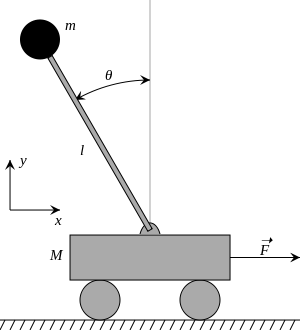
\includegraphics[width=0.4\textwidth]{Lab_report/pics/modelBuilding/300px-Cart-pendulum.svg.png}
    \caption{Sketch of the Balanbot}
    \label{fig:balanbot_sketch}
\end{figure}
% Please add the following required packages to your document preamble:
% \usepackage[table,xcdraw]{xcolor}
% If you use beamer only pass "xcolor=table" option, i.e. \documentclass[xcolor=table]{beamer}
\begin{table}[H]
\centering
\caption{Glossary }
\label{tab:glossary}
\begin{tabular}{|lx{1pt}l|l|}
\hline
\rowcolor[HTML]{C0C0C0} 
character      & description                                                                            & unit                     \\ \Xhline{1}
$x$            & Position of cart, may also be used as velocity: $\dot{x}$ and acceleration: $\ddot{x}$ & $m$,$^m/_s$, $^m/_{s^2}$ \\ \hline
$\Phi$         & pendulums position                                                                     & degree                   \\ \hline
$m_{cart}$     & Mass of the cart                                                                       & kg                       \\ \hline
$m_{pendulum}$ & Mass of the pendulum                                                                   & kg                       \\ \hline
$\mu$          & friction coefficient                                                                   & .                        \\ \hline
$I$            & moment of inertia                                                                      & $^m/_{s^2}$               \\ \hline
$F$            & Force generated by the motors acting in the movement direction                         & N                        \\ \hline
$F_x$          & Force in horizontal direction acting between pendulum and cart                         & N                        \\ \hline
$F_y$          & Force in vertical direction acting between pendulum and cart                           & N                        \\ \hline
$F_r$          & Friction force acting against the movement direction of the cart                       & N                        \\ \hline
$g$            & Gravitational Constant                                                                 & $^m/_{s^2}$               \\ \hline
$l$            & Length of pendulum                                                                     & $m$                      \\ \hline
$x_G$           &Distance in x-direction of the pendulum to the center of gravity of the system         &$m$                        \\ \hline
$y_G$           &Distance in y-direction of the pendulum to the center of gravity of the system         &$m$                        \\ \hline
$b$            &coefficient for F\textsubscript{r}                                                      & $\frac{kg}{s}$                      \\ \hline
\end{tabular}
\end{table}

\section{Model development}
The four base equations of the system have been derived from the sketch shown in \autoref{fig:forces}.

\begin{figure}[H]
    \centering
    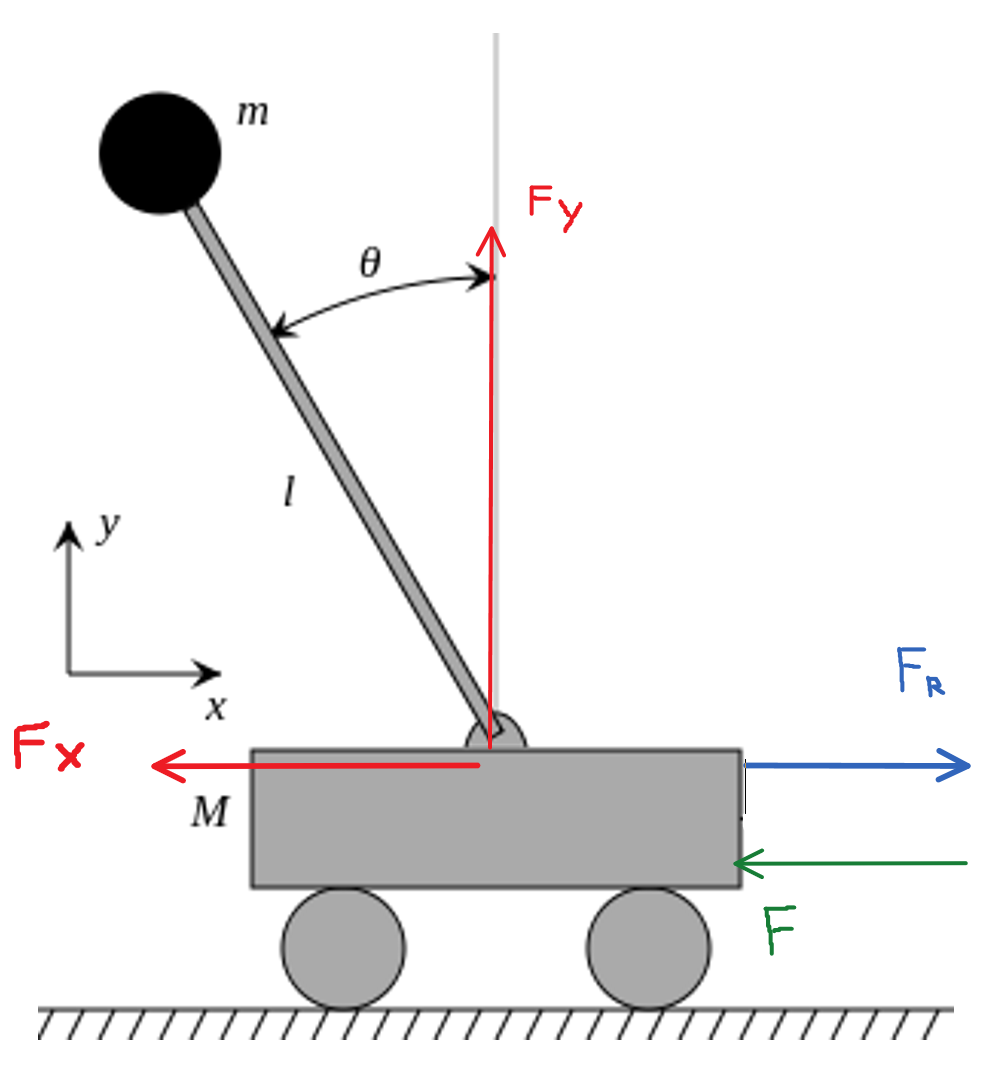
\includegraphics[width=0.4\textwidth]{Lab_report/pics/modelBuilding/forces.png}
    \caption{Sketch of the Balanbot, forces included}
    \label{fig:forces}
\end{figure}

    \begin{align}    \label{eq: base 1 (a)}
        a = \ddot{x} = \frac{\sum F}{m_{cart}} = \frac{F-F_x-F_r}{m_{cart}}
    \end{align}

    \begin{align}    \label{eq: base 2 (alpha)}
            \ddot{\Phi} = \alpha = \frac{\sum T}{I} = \frac{F_x(cos(\Phi)-F_y sin(\Phi))}{I}
    \end{align}

    \begin{align}   \label{eq: base 3 (F_x)}
        F_x = m_{pendulum} \cdot \ddot{x_G} \notag\\
        x_G = x + l sin(\Phi)\notag \\
        \dot{x_G} = \dot{x} + l \dot{\Phi} cos(\Phi)\notag \\
        \ddot{x_G} = \ddot{x} - l \dot{\Phi} sin(\Phi) + l \ddot{\Phi} cos(\Phi)\notag \\ \cline{1-2}
        F_x = m_{pendulum}\cdot(\ddot{x} - l \dot{\Phi} sin(\Phi) + l \ddot{\Phi} cos(\Phi))
    \end{align}
 
    \begin{align}   \label{eq: base 4 (F_y)}
        F_y = m_{pendulum} \cdot (\ddot{y_G} + g)\notag \\
        y_G = l  cos(\Phi)\notag \\
        \dot{y_G} = -l  \dot{\Phi}  sin(\Phi)\notag \\
        \ddot{y_G} = -l \dot{\Phi}^2  cos(\Phi) - l \ddot{\Phi} sin(\Phi)\notag \\\cline{1-2}
        F_y = m_{pendulum} \cdot (g - l \dot{\Phi}^2  cos(\Phi) - l \ddot{\Phi} sin(\Phi))
    \end{align}
    After deriving the base equations from the system, the next goal is to merge the equations and receive final equations in the following form: $\ddot{x} = \dots$ and $\ddot{\Phi} = \dots$. The first final equation describes the acceleration of the system, the other one the angle of the pendulum. To receive this form, \autoref{eq: base 3 (F_x)} gets inserted into \autoref{eq: base 1 (a)}.
    
    \begin{align}\label{eq: final eq for x ddot}
        \ddot{x} \cdot m_{cart} = F-m_{pendulum}(\ddot{x}-l\dot{\Phi}^2 sin(\Phi)+l \ddot{\Phi} cos (\Phi))-\underbrace{b\dot{x}}_\text{F\textsubscript{r}})\notag \\
         \ddot{x} m_{cart} = F-m_{pendulum}\cdot\ddot{x}+m_{pendulum}l\dot{\Phi}^2 sin(\Phi)-m_{pendulum}l\ddot{\Phi}cos(\Phi)-b\dot{x}\notag \\
         \ddot{x}(m_{cart}+m_{pendulum})+b\dot{x}=F+m_{pendulum}l\dot{Phi}^2 sin(\Phi)-m_{pendulum}l\ddot{\Phi}cos(\Phi)\notag \\\notag \\\hline \notag \\
         \ddot{x} = \frac{F+m_{pendulum}l\dot{\Phi}^2 sin(\Phi)-m_{pendulum}l\ddot{\Phi}cos(\Phi)-b\dot{x}}{m_{cart}+m_{pendulum}}
    \end{align}
    \\
    To obtain $\ddot{\Phi} = \dots$, \autoref{eq: base 3 (F_x)} and \autoref{eq: base 4 (F_y)} get inserted into \autoref{eq: base 2 (alpha)}:
    \begin{align} \label{eq: final eq for Phi ddot}
        \ddot{\Phi} I = m_{pendulum} (\ddot{x} - l\dot{\Phi}^2 sin(\Phi) + l\ddot{\Phi} cos(\Phi))\cdot lcos(\Phi)-m_{pendulum}(g-l-\dot{\Phi}^2 cos(\Phi)-l\ddot{\Phi}sin(\Phi))\cdot l\sin(\Phi)\notag \\\notag\\
        \ddot{\Phi} I = m_{pendulum} l cos(\Phi) \ddot{x} \cancel{- m_{pendulum} l^2 cos(\Phi) sin(\Phi) \dot{\Phi}^2} + m_{pendulum} l^2 cos^2(\Phi) \ddot{\Phi} - m_{pendulum}g l sin(\Phi) \dots \notag\\ \dots \cancel{+m_{pendulum}l^2 sin(\Phi)cos(\Phi)\dot{\Phi}^2}+m_{pendulum}l^2 sin^2(\Phi)\ddot{\Phi}\notag \\\notag \\
        \ddot{\Phi} I = m_{pendulum} l cos(\Phi) \ddot{x} + m_{pendulum} l^2 \ddot{\Phi} (\underbrace{cos^2(\Phi)+sin^2(\Phi)}_\text{= 1})-m_{pendulum} g l sin(\Phi)\notag \\
         \ddot{\Phi} I + m_{pendulum}l^2\ddot{\Phi} = m l cos(\Phi)\ddot{x} + m_{pendulum} g l sin(\Phi)\notag \\\cline{1-2}\notag \\
         \ddot{\Phi} = \frac{m_{pendulum}\cdot lcos(\Phi)\ddot{x}+m_{pendulum}\cdot glsin(\Phi)}{I+m_{pendulum}\cdot l^2}
    \end{align}

\subsection{Consequence for the placement of the battery}
The first discussion point should revolve around what physically happens when the battery is placed lower, or higher on the balanbot. As the battery moves further from the axles center (note: the battery generates around xx\% of the balanbots mass), the moment of inertia increases too (\cite{enwiki:satz_von_steiner}). Also the center of gravity moves up the balanbot. This leads to a more unstable system, which means on the one hand, that the actors get more authority over the balanbot, but on the other, that the controller, needs to be tuned to a faster reaction time. One additional factor which lead to this decision was the less than ideal behaviors of the half bridge and the geared motors. 

So after considering all these factors, the battery was placed on the lower possible position (\autoref{fig:lower_bat_pos}).

\subsection{Model of the system}
In this next step, the Model was transferred to Matlab Simulink and tested. For further used this was done using submodels. Which doesn't alter the results and conclusion which are derived of this simulation.
\begin{figure}[H]
    \centering
    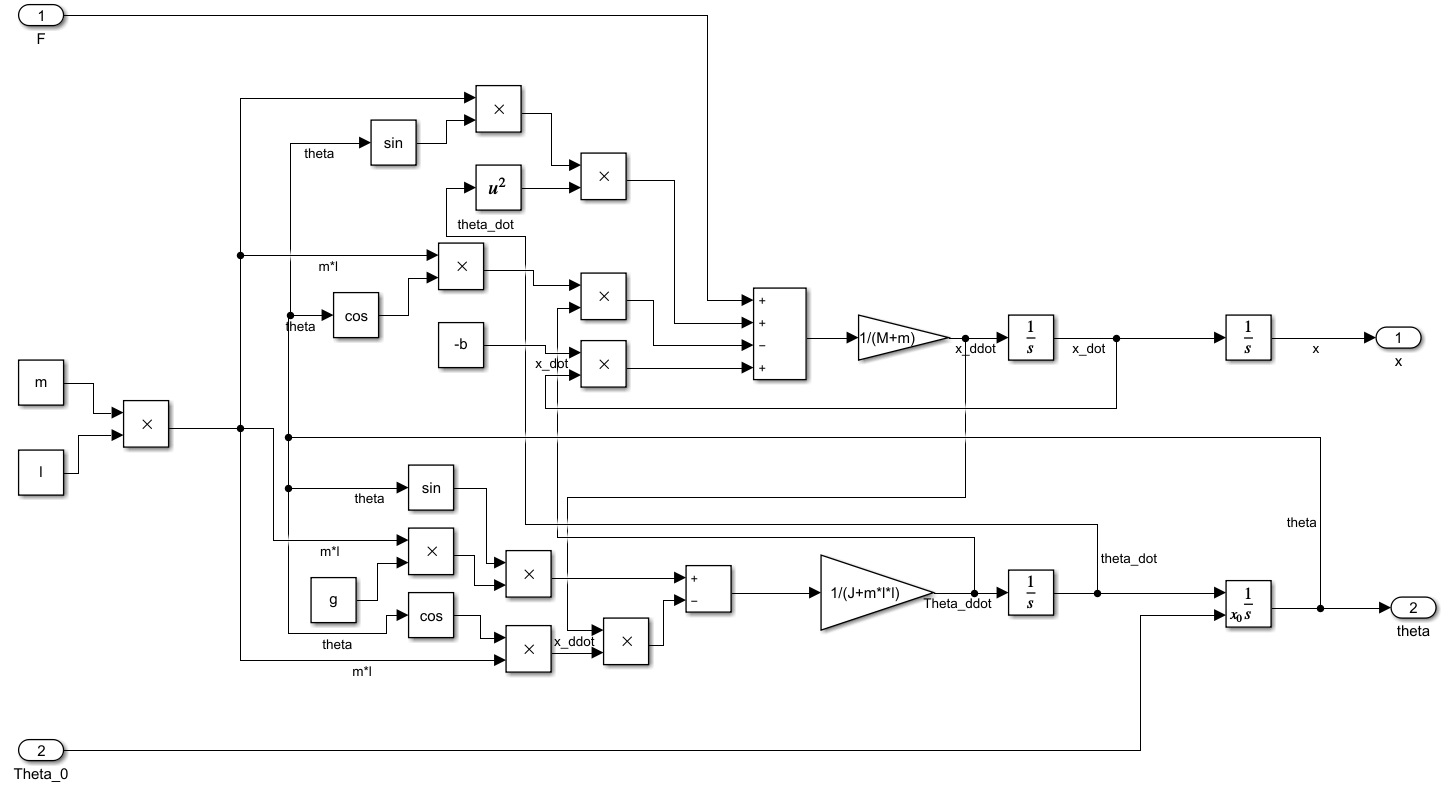
\includegraphics[width=0.8\textwidth]{Lab_report/pics/modelBuilding/non_linearized_model.PNG}
    \caption{Simulink Subsystem of non linearized model}
    \label{fig:non_linearized_model}
\end{figure}
\subsection{Analysis of the System}
\subsubsection{theta = 0}
The first part of analysis of our system was to test the behavior of the system when no Force is put on the cart and the pendulum is completely upright when starting.

In the \grqq real world \grqq it would be expected, that the pendulum will begin to fall in a considerably small time (Maybe a few seconds of upright position). This may come from small air movements around the pendulum, an unprecise placement of the pendulum, or more relativistic effects (like brownian particle movement). 

However since these before mentioned interferences weren't modeled in Simulink the pendulum should remain completely upright when simluting under these circumstances. 
\begin{figure}[H]
    \centering
    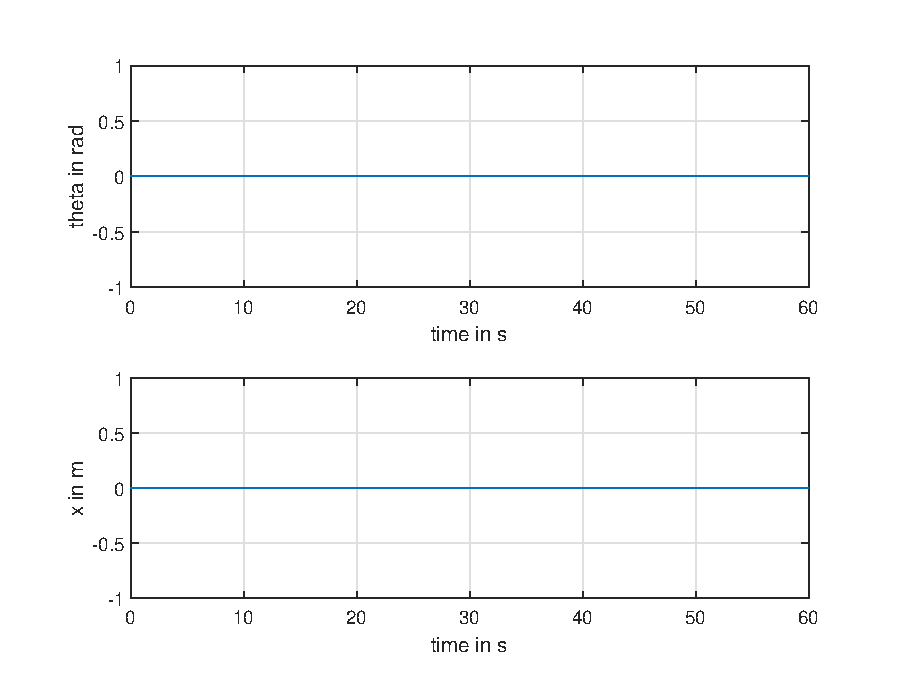
\includegraphics[width=0.8\textwidth]{Lab_report/pics/plots/non_linearized_results_theta_0.eps}
    \caption{Simulation results non-linearized model, $\Theta=0$}
    \label{fig:sim_res_non_lin_t_0}
\end{figure}

As can be seen in \autoref{fig:sim_res_non_lin_t_0}, the model behaves exactly as expected. The pendulum remains upright and the cart is not moving. For that matter: Complete success

\subsubsection{theta=5}
The next step was to test the model with an initial angle of $\Theta=5^\circ$. In comparison to the last scenario now the pendulum should not remain upright, but should slowly begin to swing. Due to the simulated friction the amplitude of the swinging should decay by time.

\begin{figure}[H]
    \centering
    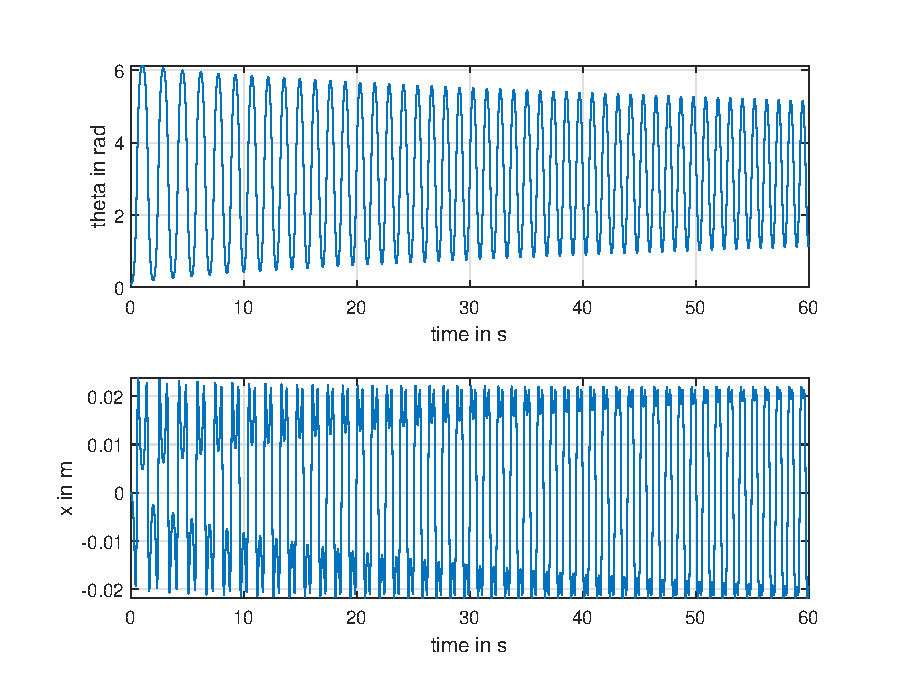
\includegraphics[width=0.8\textwidth]{Lab_report/pics/plots/non_linearized_results_theta_5.eps}
    \caption{Simulation results non-linearized model, $\Theta=5^\circ$}
    \label{fig:sim_res_non_lin_t_5}
\end{figure}
To make the amplitude decay even clearer, and to exclude all other causes of this decay, one more simulation was made. Now the factor for the friction was increased by a factor of 6, to result in $b=0.6$. All other parameters of the simulation remained the same. 
\begin{figure}[H]
    \centering
    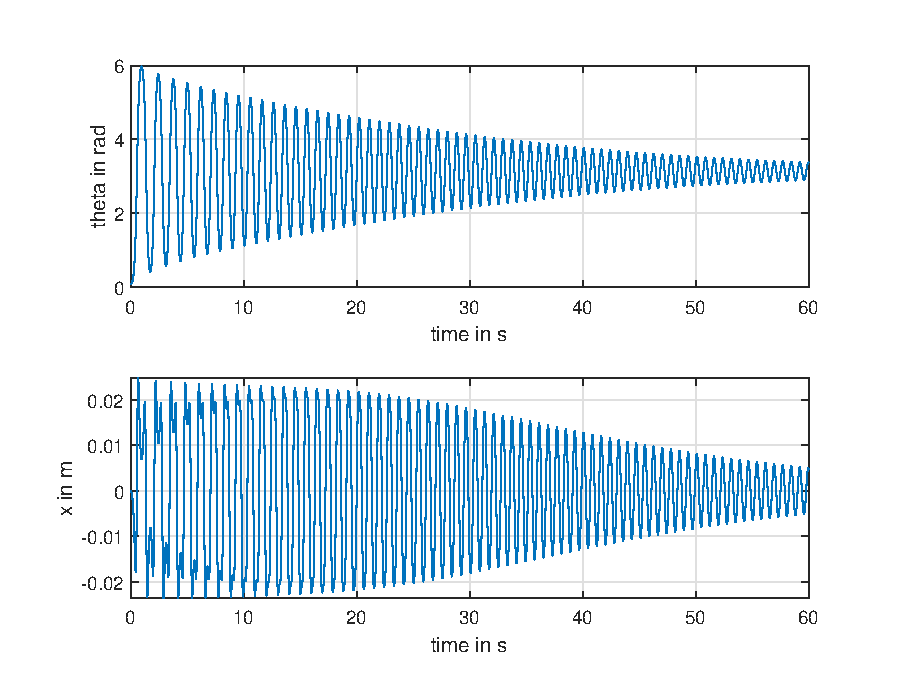
\includegraphics[width=0.8\textwidth]{Lab_report/pics/plots/non_linearized_results_inc_friction.eps}
    \caption{Simulation results non-linearized model, $\Theta=5^\circ$}
    \label{fig:sim_res_non_lin_t_5_inc_fric}
\end{figure}
The increased rate of decay can be observed very clearly in \autoref{fig:sim_res_non_lin_t_5_inc_fric}.

\section{Linearization}
To explain the step of Linearization our first step is to show which parts of our function are not linear. According to an general definition of Linearity, linearity describes the property of a system to always respond to a change in one parameter with a proportional change in another parameter (\cite{dewiki:Linearity}). This is not true for sine and cosine functions. These are not linear. Per se this isn't a problem, but it can make some future steps and simulations a lot easier if these function were replaced by a different expression.

A general approach to linearising these functions is the development of a Taylor Polynom with varying degree (The higher the degree of the Polynome, the preciser the approximation). In our specific case we have the added bonus of only using very small angles. When looking closely at the course of the function (\autoref{fig:sine_cos}), it can be seen that the sine and cosine functions at very low angles can also be calculated without the development of a Taylor series (better: only using the first factor of the Taylor series) to estimate the value. The error resulting of this process will be discussed in a future chapter(see \autoref{ssection:Comparison_lin_non_lin}).
\begin{figure}[H]
    \centering
    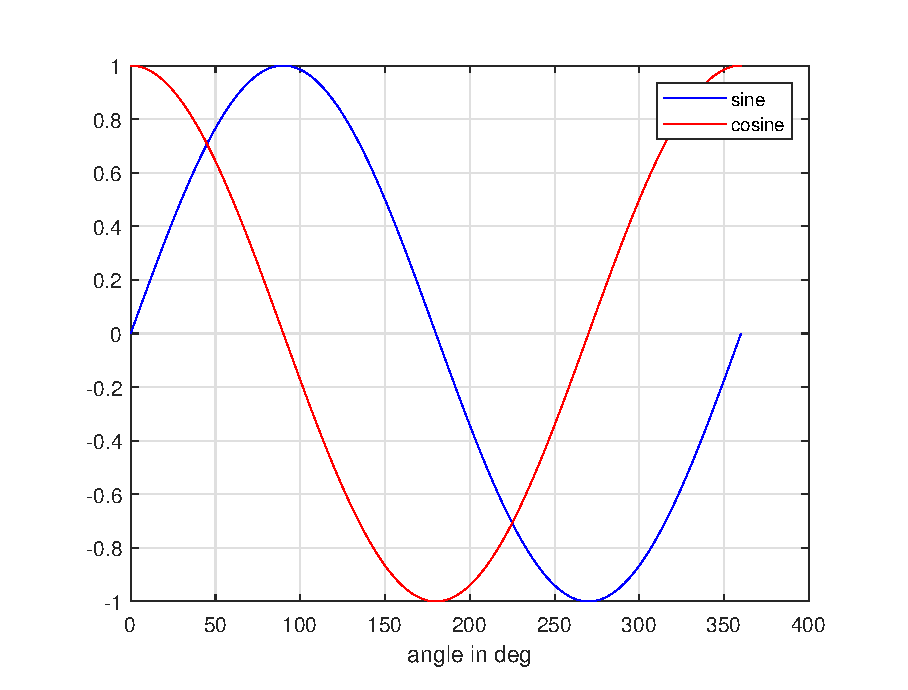
\includegraphics[width=0.8\textwidth]{Lab_report/pics/plots/sin_cos.eps}
    \caption{plot of sine and cosine}
    \label{fig:sine_cos}
\end{figure}
\subsection{Excursus Taylorseries}
To further explain how the before mentioned non-linear functions can be replaced, the Taylor Series will be developed for both. The general definition of the Taylor Series is:
\begin{equation}
      T_{f(x;a)} = \sum^\infty_{n=0} \frac{f^{(n)}(a)}{n!}(x-a)^n
    \label{eq:Taylor_Series}  
\end{equation}
\subsubsection{Sine Function}
To get the corresponding values for the Linerization it was decided to get the developed Taylor series from a collection of formulas(\cite{papula2017mathematische}).
\begin{align}
    \sin \,(x)&=\sum _{n=0}^{\infty }(-1)^{n}{\frac {x^{2n+1}}{(2n+1)!}} \\
    &=x-{\frac {x^{3}}{6}}+{\frac {x^{5}}{120}}-\cdots \cite[p. 187]{papula2017mathematische}
\end{align}
Since the development of the series stops at the first term, the linearized version of the $\sin(x)$ is $x$.
\subsubsection{Cosine Funktion}
\begin{align}
    cos(x)&=\sum _{n=0}^{\infty }(-1)^{n}{\frac {x^{2n}}{(2n)!}}\\
    &=1-{\frac {x^{2}}{2}}+{\frac {x^{4}}{24}}-\cdots  \cite[p. 187]{papula2017mathematische}
\end{align}

Since the development of the series stops at the first term, the linearized version of the $\cos(x)$ is $1$.
\subsection{Simulink Model}
The linearization of the before developed Matlab model is a fast and easy step. In that our case we just replaced the sine and cosine Blocks with the corresponding gains. 

\section{Comparison of linear vs. non-linear System}
\label{ssection:Comparison_lin_non_lin}

\section{System Analysis with Transfer Function}

Open loop response with no offset
Open loop response with initial condition $\Phi = 5^\circ$

\chapter{Controller Development}
\section{Proportional Gain}
In a first approach in controlling this system a proportional gain was installed. The gain will be used in further sections to find the parameters for a PID controller by using the Ziegler-Nichols method.
\begin{figure}
    \centering
    \begin{subfigure}{0.45\textwidth}
        \includegraphics[]{}
    \end{subfigure}    
    \caption{Caption}
    \label{fig:my_label}
\end{figure}

\chapter{Hardware Implementation}
\section{Task Clarification}
Until now a model was developed and with this model settings for a PID controller were found. To test these settings on the real BalanBot, a Simulink model which implements the hardware specific functions is needed. This includes reading the acceleration and gyroscope sensors, filtering and processing them and writing to the output registers. This ensures that the BalanBot also moves in a different direction with a negative output of the controller than with a positive output. 

\section{Detailed Code Commentary}
\subsection{Sensor Data Reading}
The IMU communicates with the Arduino via the I2C bus. This must be implemented in the Simulink design. The sensor values obtained from this must now be further ground via Matlab function blocks. To get more trustworthy data in the later course of the program, a Kalman filter was also used. However, this filter needs both the measured angle and the measured yaw rate for proper operation. Therefore these two values were calculated. 

\begin{figure}[H]
    \centering
    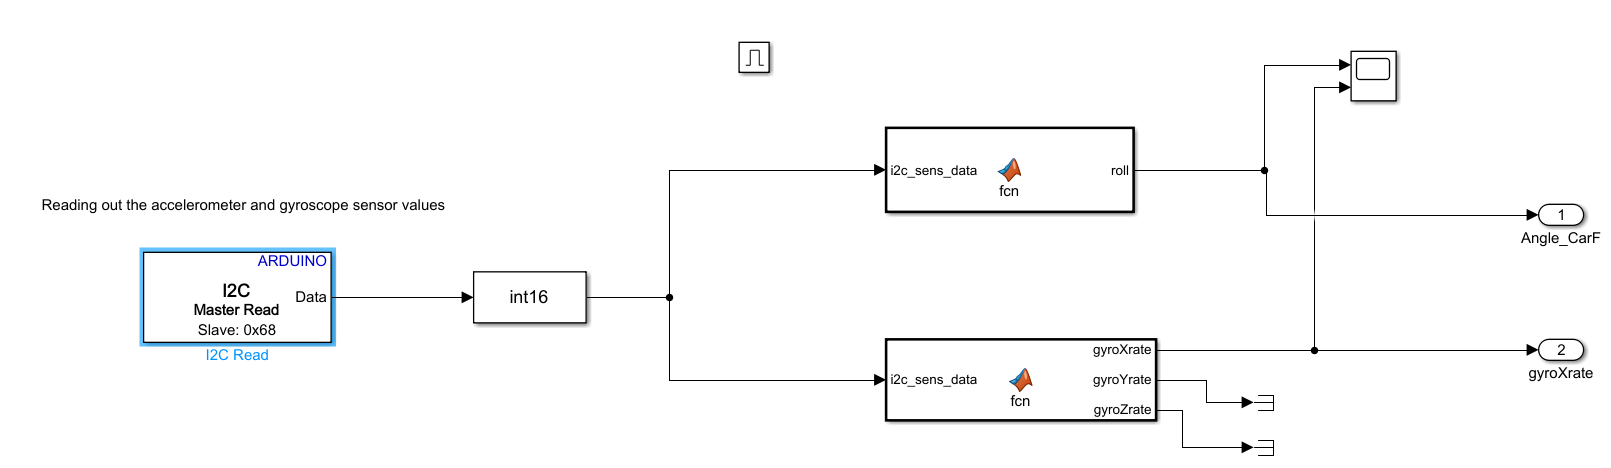
\includegraphics[width=\textwidth]{Lab_report/pics/hardware_impl/gyro_read.PNG}
    \caption{data reading Submodel}
    \label{fig:acc_gyro_read}
\end{figure}

\begin{lstlisting}[language=Matlab, caption=angle calculation]
function roll = fcn(i2c_sens_data)
    accX = double(i2c_sens_data(1));
    accY = double(i2c_sens_data(2));
    accZ = double(i2c_sens_data(3));
    roll = atan(accY / sqrt(accX * accX + accZ * accZ)) * 180/pi; 
end
\end{lstlisting}

\begin{lstlisting}[language=Matlab, caption=gyro rate calculation]
function [gyroXrate,gyroYrate,gyroZrate] = fcn(i2c_sens_data)
    gyroX = double(i2c_sens_data(5));
    gyroY = double(i2c_sens_data(6));
    gyroZ = double(i2c_sens_data(7));
    gyroXrate = gyroX/131;
    gyroYrate = gyroY/131;
    gyroZrate = gyroZ/131; 
end
\end{lstlisting}

\subsection{Data Processing}
In this submodel, the determined data is first filtered by a Kalman filter and then fed to the control algorithm. The data processing by means of this filter is described in more detail below.
\subsubsection{Kalman filter}
The principle of this filter is based on the estimation of the output quantity and the comparison of the measured output quantity. The difference of these two quantities is then weighted with the Kalman gain and used to correct the estimated output value. In our case the code for this estimation and correction algorithm is already finished and only a small test and proof of concept will be shown here. 

\subsubsection{Controller}
To control the BalanBot, a PID controller was implemented after the Kalman filter.
\begin{figure}[H]
    \centering
    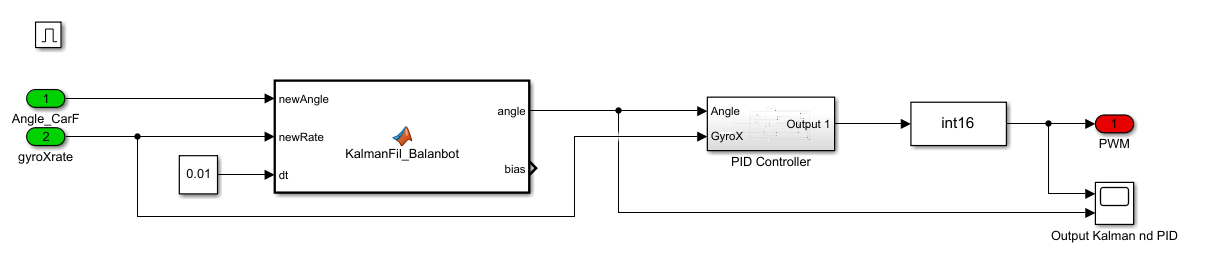
\includegraphics[width=\textwidth]{Lab_report/pics/hardware_impl/motor-control.PNG}
    \caption{Model of the Motor Control}
    \label{fig:motor control model}
\end{figure}

The PID-Controller Submodel looks as can be seen in \autoref{fig:pid_model}.
\begin{figure}[H]
    \centering
    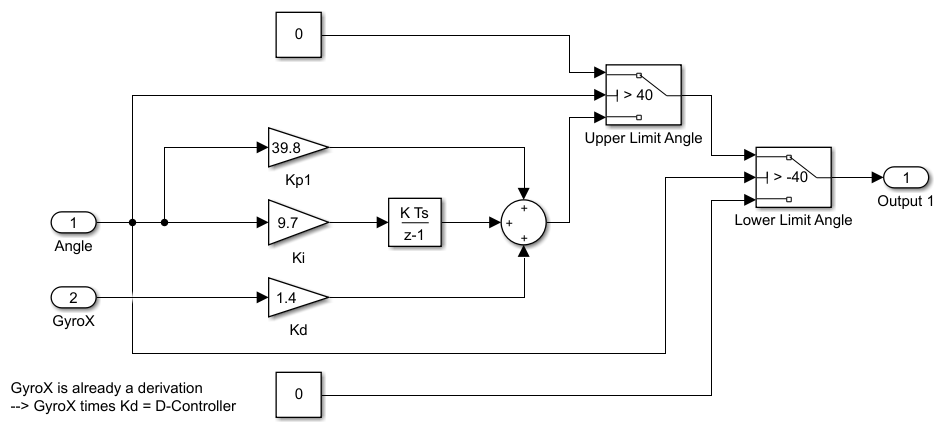
\includegraphics[width=\textwidth]{Lab_report/pics/hardware_impl/PID.PNG}
    \caption{Model of the PID Controller}
    \label{fig:pid_model}
\end{figure}
To 
The angle limit was also implemented into the PID-Controller Submodel. If the angle of the BalanBot is bigger than $40^\circ$ or smaller than $-40^\circ$ , the output (= motor speed) gets set to 0RPM.
\newline\\\\
\textbf{Adjusting of the PID-Controller gains}\\
The settings of the PID controller had already been estimated by using the Simulink model beforehand. However, when testing these settings on the real BalanBot, the PID-Controller could not stabilize the BalanBot.\\\\
To obtain some reasonable PID-Controller parameter values, all gains have been initially set to zero. Then, the proportional gain was estimated at first. To get rid of the steady-state-error, a integral gain was also estimated and implemented. However, the BalanBot reacted way too aggressive to faster errors, hence a derivative gain was estimated and implemented.\\\\
The fine tuning of the controller was done in the following order:
\begin{itemize}
    \item Adjusting the proportional gain until the outcome was somewhat nearly satisfactory
    \item Adjusting the integral gain in combination with the proportional gain so the BalanBot would react fast enough but not too strong to errors
    \item Adjusting the derivative gain to smooth the aggressiveness of the controller
\end{itemize}

The final PID-Controller gains can be seen in \autoref{fig:pid_model}.
\subsection{Motor Control}


\chapter{Tests and Validation}
A video of the working BalanBot can be viewed by scanning the QR-code below or simply following this link: \url{https://www.youtube.com/watch?v=ocpmd9iVG38}
\begin{figure}[H]
    \centering
    
\includegraphics[width=0.25\textwidth]{Lab_report/pics/testvalid/frame.png}
    \caption{QR-Code linking a youtube-video of the working BalanBot}
    \label{fig:balanbot_qe}
\end{figure}

\newpage
\chapter{Signaturen}
    Fertig gestellt am \today \\
    \begin{figure}[H]
        \centering
        
\includegraphics{LaTeX/pics/signature_grebien.png}
    	\caption{Signatur: Grebien Alexander}
    	\label{pic:signatur_grebien}
    \end{figure}
        
\listoffigures
\listoftables
\bibliographystyle{ieeetr}
\bibliography{meine_Zitatsbibliothek.bib}
\end{document}
